\begin{figure}[ht]
	\begin{center}
		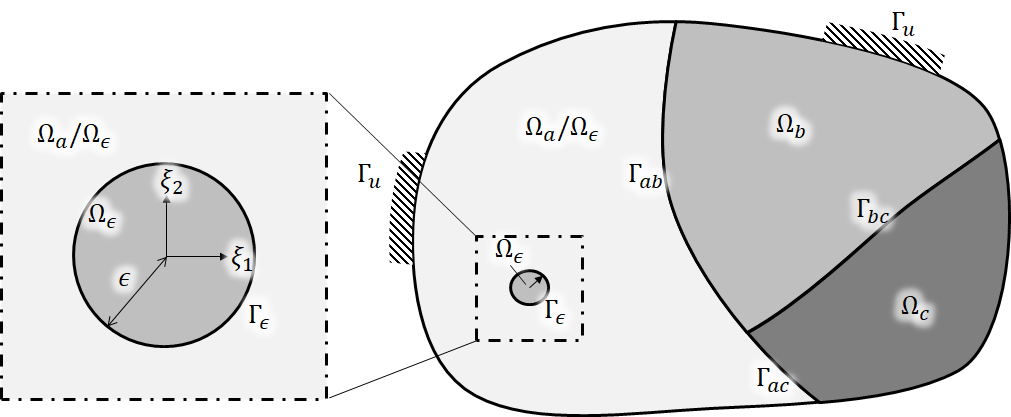
\includegraphics[width=13cm]{./figures/TD.png}
		\caption{Topological derivative}
		\label{fig:TD}
	\end{center}
\end{figure}

objective function
\begin{align}
\min_{\Omega_1,\Omega_2}F=-\Bigr(\sum_{p=1}^{n}\frac{1}{\lambda_p}\Bigl)^{-1}
\end{align}


状態方程式は以下のようになる。
\begin{align}
	&C_{ijkl}^{p}u_{k,lj}^{}+\lambda\rho^{p} u_{i}=0&\text{in}\hspace{0.3cm}\Omega_{p}
	\label{eq:govmain}
	\\
	&u_{i}=0 &\text{on}\hspace{0.3cm}\Gamma_{D}
	\\
	&C_{ijkl}u_{k,l}^{}n_{j}=0 &\text{on}\hspace{0.3cm}\Gamma_{N}
	\\
	&u_{i}^{p}=u_{i}^{p} &\text{on}\hspace{0.3cm}\Gamma_{pq}
	\\
	&C_{ijkl}^{p}u_{k,l}^{p}n_{j}^{p}+C_{ijkl}^{q}u_{k,l}^{q}n_{j}^{q}=0 &\text{on}\hspace{0.3cm}\Gamma_{pq}
	\label{eq:govbc}
	\\
	&\sum_{p=1}^{n}\int_{\Omega_p}(\rho^{p}u_{i}u_{i}) d\Omega=1
	\label{eq:govnorm}
\end{align}

ラグラジアンを以下のように定式化する。
\begin{align}
	\mathscr{L}(\Omega_{p\{1\leq p\leq n\}};\bm{U},X,\bm{V},Y)=
	&X+\sum_{p=1}^{n}\int_{\Omega_p}\Bigr( V_{i,j}C_{ijkl}^{p}U_{k,l}-X\rho^{p}V_{i}U_{i}\Bigl) d\Omega
	\nonumber
	\\
	&-\sum_{p=1}^{n-1}\sum_{p=q}^{n}\int_{\Gamma_{pq}}\frac{1}{2}\Bigr(C_{ijkl}^{p}U_{k,l}^{p}n_{j}^{p}-C_{ijkl}^{q}U_{k,l}^{q}n_{j}^{q}\Bigl)(V_{i}^{p}-V_{i}^{q}) d\Gamma
	\nonumber
	\\
	&-\sum_{p=1}^{n-1}\sum_{p=q}^{n}\int_{\Gamma_{pq}}\frac{1}{2}\Bigr(V_{i,j}^{p}C_{ijkl}^{p}n_{l}^{p}-V_{i,j}^{q}C_{ijkl}^{q}n_{l}^{q}\Bigl)(U_{k}^{p}-U_{k}^{q})d\Gamma
	\nonumber
	\\
	&-\sum_{p=1}^{n}\int_{\Gamma_{pu}}\Bigr(C_{ijkl}^{p}U_{k,l}^{p}n_{j}^{p}\Bigl)(V_{i}^{p}) d\Gamma
	\nonumber
	\\
	&-\sum_{p=1}^{n}\int_{\Gamma_{pu}}\Bigr(V_{i,j}^{p}C_{ijkl}^{p}n_{l}^{p}\Bigl)(U_{k}^{p}) d\Gamma
	\nonumber
	\\
	&+Y\Bigr\{1- \sum_{p=1}^{n}\int_{\Omega_{p}}(\rho^{p}U_{i}U_{i}) d\Omega \Bigl\}
	\label{eq:lagrange}
\end{align}
ここで,$\bm{U},X$はそれぞれ状態変数$\bm{u},\lambda$に対応する設計変数,$\bm{V},Y$はラグランジュ乗数である。
ただし,$\bm{u}$や$\lambda$が領域$\Omega_p$に依存する関数であるのに対し,$\bm{U},X,\bm{V},Y$は$\Omega_p$に依存しない関数である。

ラグラジアン\eqref{eq:lagrange}に対し,$\bm{V}$に関して部分積分を行うと
\begin{align}
	\mathscr{L}(\Omega_{p\{1\leq p\leq n\}};\bm{U},X,\bm{V},Y)=&X-\sum_{p=1}^{n}\int_{\Omega_p}\Bigr(C_{ijkl}^{p}U_{k,lj}+X\rho^{p}U_{i}\Bigl)V_{i} d\Omega
	\nonumber
	\\
	&+\sum_{p=1}^{n-1}\sum_{p=q}^{n}\int_{\Gamma_{pq}}\frac{1}{2}\Bigr(C_{ijkl}^{p}U_{k,l}^{p}n_{j}^{p}+C_{ijkl}^{q}U_{k,l}^{q}n_{j}^{q}\Bigl)(V_{i}^{p}-V_{i}^{q}) d\Gamma
	\nonumber
	\\
	&-\sum_{p=1}^{n-1}\sum_{p=q}^{n}\int_{\Gamma_{pq}}\frac{1}{2}\Bigr(V_{i,j}^{p}C_{ijkl}^{p}n_{l}^{p}-V_{i,j}^{q}C_{ijkl}^{q}n_{l}^{q}\Bigl)(U_{k}^{p}-U_{k}^{q})d\Gamma
	\nonumber
	\\
	&+\sum_{p=1}^{n}\int_{\Gamma_{pN}}\Bigr(C_{ijkl}^{p}U_{k,l}^{p}n_{j}^{p}\Bigl)(V_{i}^{p}) d\Gamma
	\nonumber
	\\
	&-\sum_{p=1}^{n}\int_{\Gamma_{pu}}\Bigr(V_{i,j}^{p}C_{ijkl}^{p}n_{l}^{p}\Bigl)(U_{k}^{p}) d\Gamma
	\nonumber
	\\
	&+Y\Bigr\{1- \sum_{p=1}^{n}\int_{\Omega_{p}}(\rho^{p}U_{i}U_{i}) d\Omega \Bigl\}
	\nonumber
	\\
	\label{eq:lagrange_wint}
\end{align}
状態方程式\eqref{eq:govmain}~\eqref{eq:govnorm}より,$\bm{U}=\bm{u}(\Omega_{p\{1\leq p\leq n\}})$,
$X=\lambda(\Omega_{p\{1\leq p\leq n\}})$とすれば,任意の$\bm{V},Y$に対して次式が成立することがわかる。
\begin{align}
	\mathscr{L}(\Omega_{p\{1\leq p\leq n\}};\bm{u},\lambda,\bm{U},Y)=\lambda(\Omega_{p\{1\leq p\leq n\}})
\end{align}
$\bm{V}=\bm{v}(\Omega_{p\{1\leq p\leq n\}})$,
$Y=\eta(\Omega_{p\{1\leq p\leq n\}})$

